\section{SAT/SMT-based Analysis}


\subsection{SAT Solving Algorithms}

The process of SAT solving looks as follows:
\begin{center}
	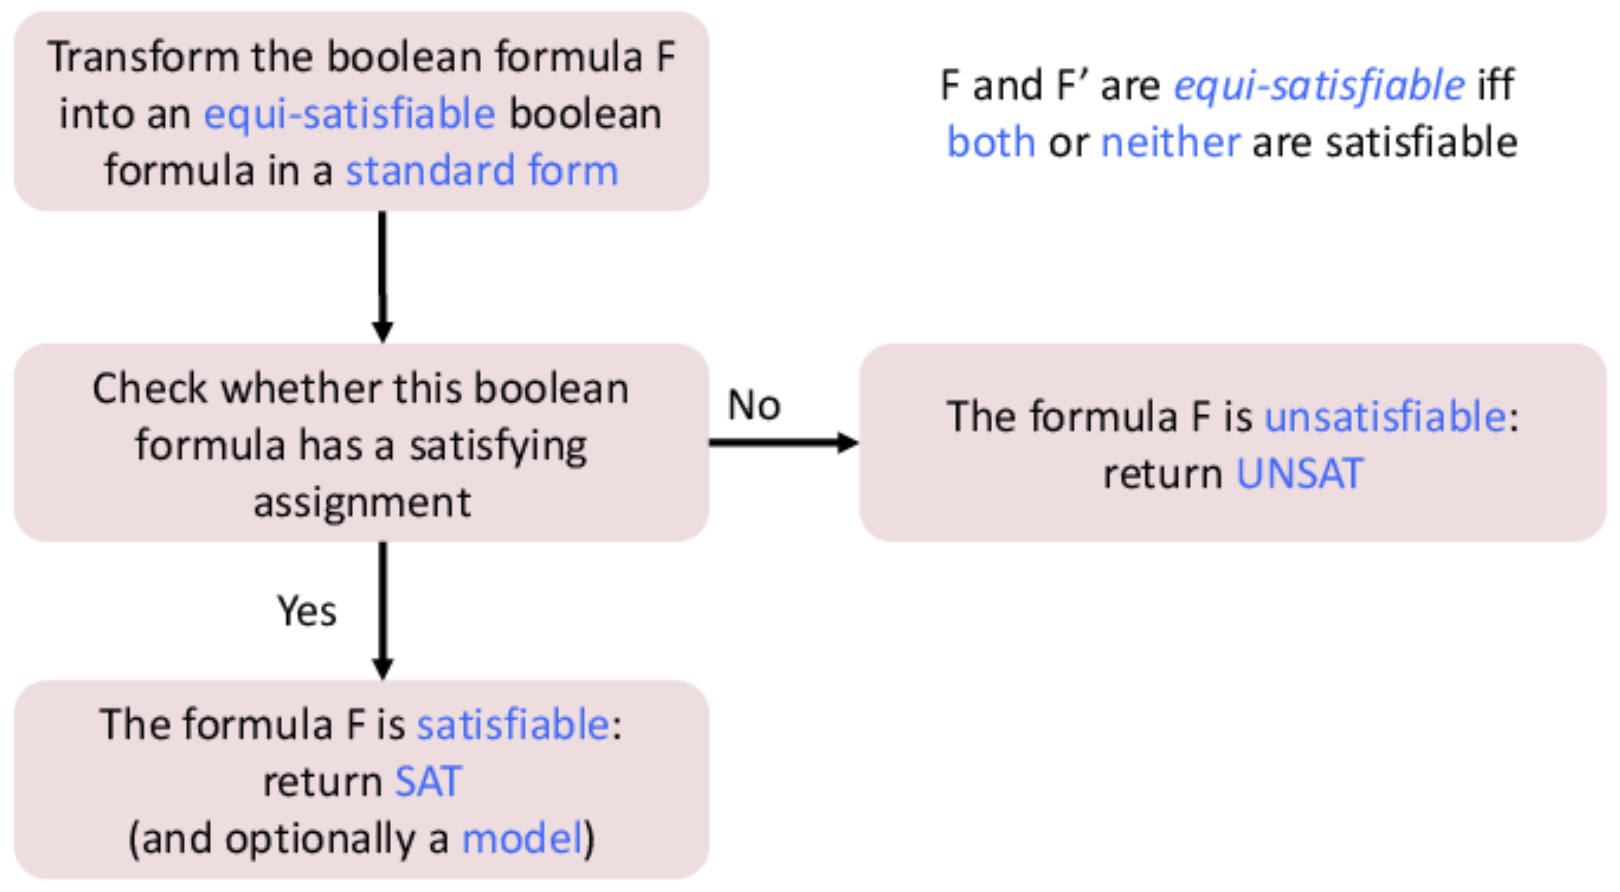
\includegraphics[width=\columnwidth]{assets/sat_solving}
\end{center}

As the standard form we use the conjunctive normal form (CNF). A formula $F$ is in CNF iff it is a conjunction of clauses. A clause is a disjunction of literals (a literal being a variable or its negation). A formula in CNF cloud look like this:
$$(p \vee \neg q) \wedge (q \vee r \vee \neg p) \wedge (s \vee p)$$

Simple conversion to CNF works as follows:
\begin{enumerate}
	\item Rewrite all $A \Rightarrow B$ to $\neg A \vee B$ and $A \Leftrightarrow B$ to $(\neg A \vee B) \wedge (A \vee \neg B)$
	\item Push all negations inwards
	\item Rewrite all $\neg \neg A$ to $A$
	\item Eliminate $\top$ and $\bot$
	\item Distribute disjunctions over conjunctions, e.g. rewrite $A \vee (B \wedge C)$ to $(A \vee B) \wedge (A \vee C)$
	\item Remove duplicate clauses and duplicate literals from clauses
\end{enumerate}

The CNF formula can be rewritten until the set is empty or a clause is empty, by using the Davis-Putman-Logemann-Loveland (DPLL) Algorithm. If the set is empty return SAT (and a model $M$, if a clause is empty return UNSAT. The rules are as follows:
\begin{itemize}
	\item Pure Literal: If $p$ occurs only positively in $F$, delete the clauses in which $p$ occurs, $M = M \cup \{p\}$ (similar if $p$ only occurs negatively.
	\item Unit propagation: If $u$ is a unit clause in $F$, delete the clauses in which $u$ occurs, update all clauses containing $\neg u$ as a disjunct by removing that disjunct, $M = M \cup \{ u \}$.
	\item Decision: If $p$ occurs both positively and negatively in F: 
	\begin{itemize}
		\item apply the algorithm to $F \wedge p, M \cup \{p\}$: if we get (SAT, $M$) then return this result
		\item otherwise, apply the algorithm to $F \wedge \neg p, M \cup \{ \neg p\}$ and return the result
	\end{itemize}
\end{itemize}


\subsection{Encoding Integers into SAT}

Alloy supports integers. Bounded integers are encoded using bit-blasting. The idea is that a 32-bit integer is a sequence of 32 individual bits. This is similar to how a circuit defines integer operations. In Alloy the bit width defines the bound for the maximum size of an integer.


\subsection{Universal Quantifiers in SMT}

When dealing with uninterpreted (user-defined) functions, the idea is to find a candidate model $M$ for the non-quantified part of the formula $F$ and check if $M$ satisfies all the universal quantifiers from $F$. This is called Model-Based Quantifier Instantiation (MBQI). In general, termination is not guaranteed when using MBQI.
